%!TEX root = ../Master.tex

\section{Kalman filters}

The Kalman filter (KF) is a technique for filtering and prediction in linear systems. In the context of robotics the filter can be used to locate the robot and make predictions as to where the robot will reside in the next time-step.\\

The technique makes it possible to do data fusion, which is the process of combining observations from a number of different sensors to provide a robust and complete description of the environment. Robots could e.g. use radar, lidar, GPS, compass, camera, etc. for location and combining these sensor informations would result in a more complete overview of the robot and it's environment.\\

The KF consists of a basic cycle which includes making predictions and updating these predictions with actual measurement data. The filter represents it's beliefs about the state of the system as a Gaussian distribution which is characterized by two parameters: the mean value $\mu$ and the variance $\sigma^2$. Another important property of the KF and Gaussians is that they are unimodel. This means that they posses a single maximum as opposed to e.g. Monte Carlo Localization which is multimodal.\\

The formal definition of the KF algorithm is given in Algorithm \ref{alg:kf_def1}. Notice that the variance is now represented by $\Sigma_{t}$ which in higher dimensional spaces denotes a covariance matrix.

\begin{center}
\begin{minipage}{.65\linewidth}
\alglanguage{pseudocode}
\begin{algorithm}[H]
\caption{Kalman Filter}
\label{alg:kf_def1}
\begin{algorithmic}[1]
\Procedure{KalmanFilter}{$\mu_{t-1},\Sigma_{t-1},u_{t},z_{t}$}
  \State $\bar\mu_{t} = A_{t}\mu_{t-1} + B_{t}u_{t}$%\Comment{This is a comment}
  \State $\bar\Sigma_{t} = A_{t}\Sigma_{t-1}A_{t}^T + R_{t}$
  \State $K_{t} = \bar\Sigma_{t}C_{t}^T(C_{t}\bar{\Sigma}_{t}C_{t}^T+Q_{t})^{-1}$
  \State $\mu_{t} = \bar\mu_{t} + K_{t}(z_{t} - C_{t}\bar\mu_{t})$
  \State $\Sigma_{t} = (I - K_{t}C_{t})\bar\Sigma_{t}$
  \State \textbf{return} $\mu_{t}, \Sigma_{t}$
\EndProcedure
\end{algorithmic}
\end{algorithm}
\end{minipage}
\end{center}

The algorithm takes four parameters: The previous mean value and variance of the system $\mu_{t-1}$ and $\Sigma_{t-1}$, respectively, the new control-input $u_{t}$ and measurement data $z_{t}$. In line 2 the previous mean value and control-input are mapped into the new mean value $\bar{\mu_{t}}$ which is a prediction of the system state. In line 3 the variance is propagated together with the measurement noise $R_{t}$. In line 4 the Kalman gain is calculated, which is used as a weight factor in line 5 to determine the degree to which we believe in the measurement as opposed to the prediction. Lastly the variance is updated in line 6.\\

The mean value of the system could be a position, velocity, or a heading. The transition matrix $A_{t}$ applies the effects of $\mu_{t-1}$ on $\mu_{t}$, and the transition matrix $B_{t}$ applies the effects of control-input $u_{t}$ on $\mu_{t}$. The factors $R_{t}$ and $Q_{t}$ models the motion noise and measurement noise, respectively. In higher dimensional spaces these will be covariance matrices.\\

As mentioned, the KF represents its beliefs about the system, predictions and measurements, as Gaussians. An important property of the KF is that combining the predictions and the measurements increases the certainty about the system state. Gaussians has the characteristic that multiplying two Gaussians produces a new Gaussian with a variance that is smaller than the variance of both the original Gaussians, and therefore this new Gaussian will have a larger peak than the original Gaussians. The mean value of the new Gaussian will lie between the two mean values of the two original Gaussians. \\

The measurement update consists of the multiplication of the prediction and the measurement Gaussians. The equations for the new mean value and variance of the Gaussian are given in Equation \ref{eq:new_mu1} and \ref{eq:new_sigma1}, respectively.

\begin{equation}
\label{eq:new_mu1}
\mu = \dfrac{\sigma_{2}^2\mu_{1} + \sigma_{1}^2\mu_{2}}{\sigma_{2}^2 + \sigma_{1}^2}
\end{equation}
\begin{equation}
\label{eq:new_sigma1}
\sigma^2 = \left(\dfrac{1}{\sigma_{2}^2} + \dfrac{1}{\sigma_{1}^2}\right)^{-1}
\end{equation}

There is a certain degree of error involved in the motion of an object due to e.g. friction. The motion update therefore consists of moving the mean value $\mu_{t-1}$ and adding some degree of uncertainty to the Gaussian which increases the variance of the new Gaussian w.r.t the original Gaussian. The motion update turns out to be very simple and is performed by adding the mean values and variances of the Gaussians representing the posterior and priori beliefs. The equations for the motion update is giving in Equation \ref{eq:new_mu2} and \ref{eq:new_sigma2}.

\begin{equation}
\label{eq:new_mu2}
\mu = \mu_{1} + \mu_{2}
\end{equation}
\begin{equation}
\label{eq:new_sigma2}
\sigma^2 = \sigma_{1}^2 + \sigma_{2}^2
\end{equation}

\subsection{Kalman Filter example}

A simple example of the KF in a one-dimensional location scenario is given in \autoref{fig:kf_ex}. A robot moves along the horizontal axis, and the initial belief about the robots location is shown in \autoref{fig:kf_ex}(a). The bold graph in \autoref{fig:kf_ex}(b) represents measurement data obtained from e.g. GPS or distance measurements relative to objects with a known location. In the measurement update step, the initial belief is combined with the measurements, which is a product of the two Gaussians. This improved belief about the robots location is calculated using Equations \ref{eq:new_mu1} and \ref{eq:new_sigma1}. The result is the bold graph shown in \autoref{fig:kf_ex}(c). As mentioned, the mean value of this new Gaussian is located between the mean values of initial belief and the measurement and the variance of the new Gaussian is smaller than the variances of both the original Gaussians. In \autoref{fig:kf_ex}(d) the bold graph represents the prediction of the location of the robot which is calculated in line 2 of Algorithm \ref{alg:kf_def1}. \\

In the motion update step, the robot is moved along the horizontal axis by adding some control-input value to the mean value of the robot, and because movement is prone to some amount of error, the variance is added with an error value to increase the variance representing the motion update uncertainty. The bold graph in \autoref{fig:kf_ex}(e) again represents a measurement made by the robot, which is combined with the prediction resulting in the bold graph in \autoref{fig:kf_ex}(f).

\begin{figure}[H]
\centering
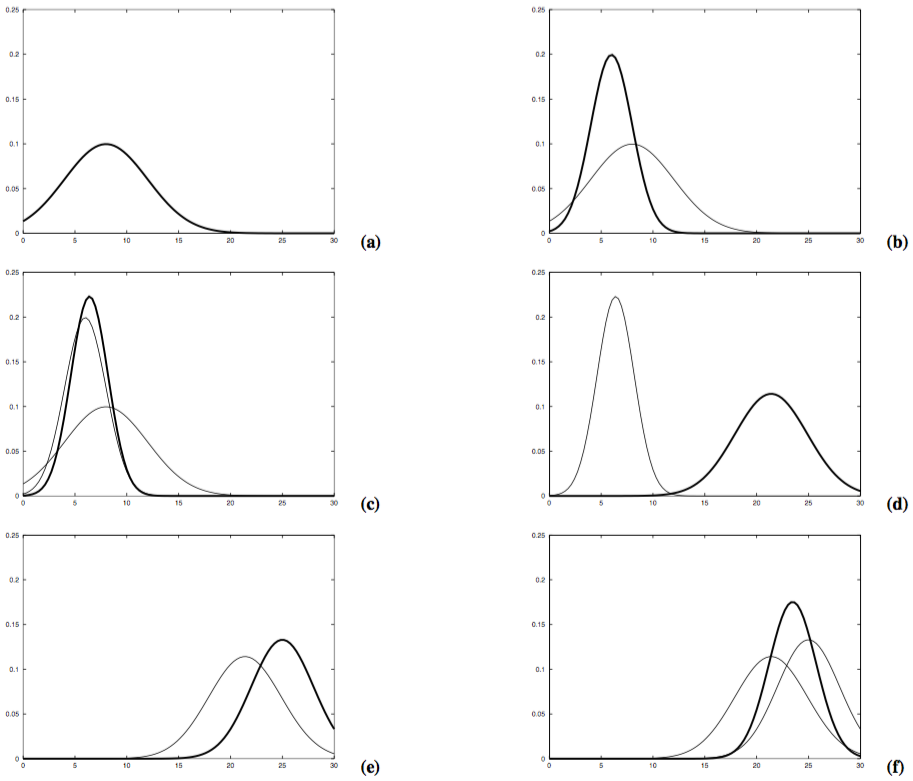
\includegraphics[scale=0.45]{images/KalmanFilterExample}
\caption{Kalman Filter example in a one-dimensional localization scenario}
\label{fig:kf_ex}
\end{figure}

\subsection{Extended Kalman filters}

The plain KF assumes that the system is linear in the state transitions and measurements with added Gaussian noise. This is however not the case in many systems and therefore the KF is inapplicable in many non-trivial problems.\\

To overcome this limitation of the plain KF, the extended Kalman Filter (EKF) can be used instead. In the EKF linearization is used to generate an approximation to the nonlinear system. This approximation to the true belief is represented by a mean value $\mu_t$ and a variance $\sigma_t^2$. Therefore the EKF represents its belief as the plain KF, but it uses an approximation instead of the exact belief.\\

The formal definition of the EKF is given in Algorithm \ref{alg:ekf_def1}.

\begin{center}
\begin{minipage}{.65\linewidth}
\alglanguage{pseudocode}
\begin{algorithm}[H]
\caption{Extended Kalman Filter}
\label{alg:ekf_def1}
\begin{algorithmic}[1]
\Procedure{ExtendedKalmanFilter}{$\mu_{t-1},\Sigma_{t-1},u_{t},z_{t}$}
  \State $\bar\mu_{t} = g(u_t,\mu_{t-1})$
  \State $\bar\Sigma_{t} = G_{t}\Sigma_{t-1}G_{t}^T + R_{t}$
  \State $K_{t} = \bar\Sigma_{t}H_{t}^T(H_{t}\bar{\Sigma}_{t}H_{t}^T+Q_{t})^{-1}$
  \State $\mu_{t} = \bar\mu_{t} + K_{t}(z_{t} - h(\bar{\mu_t}))$
  \State $\Sigma_{t} = (I - K_{t}H_{t})\bar\Sigma_{t}$
  \State \textbf{return} $\mu_{t}, \Sigma_{t}$
\EndProcedure
\end{algorithmic}
\end{algorithm}
\end{minipage}
\end{center}

The EKF in Algorithm \ref{alg:ekf_def1} looks very similar to the plain KF in Algorithm \ref{alg:kf_def1}. But the important differences are seen in line 2 and line 5, where the linear prediction of the KF are replaced by the linearized functions $g(u_t,\mu_{t-1})$ and $h(\bar{\mu_t})$, respectively. Also, the linear system matrices $A_t$ and $B_t$ have been replaced with the Jacobian $G_t$, and $C_t$ with $H_t$. The Jacobians are a consequence of the linearisation operation.
